
\chapter{Welded Braids}

Welded Braids are defined in terms of an extension of the classical braid group which described in \cref{sec:w_group}, however we will explore the flying ring visualisation of welded braids described by \cite{Bar_Natan_2016} to gain intuition.

Since welded braids can be described in numerous ways, it is also of note that welded braids can additionally be considered as a generalisation of braids into the \( 4 \)th dimension, where strands are tubes monotonically increasing in the \( w \) direction. 
This is possibly the most natural way of understanding welded braids due to it's explicit generalisation of classical braids, however, we lack the dimension to understand it completely. 

We aim to define the welded braid diagram so that we can generalise our composition operation of classical braids effectively. 
I will denote the set of welded braids with \( n \) strands as \( wB_n \) and denote the set of welded braids as \( wB \). 

\section{Visualisation of Welded Braids}

We will consider the flying rings visualisation, which is a generalisation of the movie visualisation of classical braids.
From there we will show how this is related to the welded braid group. 
And then we will consider the welded braid diagram, which we will create artificially from the welded braid group to be able to define the composition operation effectively. 

\subsection{Flying Rings Visualisation}

The flying ring visualisation is a generalisation of the movie visualisation of classical braids, where for a braid in \( wB_n \), each frame is a box \( [0, 1]^3 \) with \( n \) rings horizontal to the xy plane. 

% This visualisation is rigorously defined in terms of the welded braid group explained in \cref{sec:w_group}, however we consider this first to gain intuition. 
% However this defined in terms of the group visualisation of welded braids
% The following logic will be imprecise, however it's important to note that since this movie visualisation follows from the welded braid group described in \cref{sec:w_group}, this characterisation is inherently imprecise. 

Consider a welded braid \( B \in wB_n \).
Each frame consists within it \( n \) rings placed parallel to the xy plane in \( [0, 1]^3 \) such that at \( t = 0 \) and \( t = 1 \) each rings is linearly space along the bottom of the box on the line \( \{ (x, y, z) \in [0, 1]^3 \mid x = 1 / 2 \text{ and } z = 0 \} \)
This is similar to the classical braid definition, where the points begin and end linearly spaced in \( [0, 1]^2 \). 

We want to consider crossings between strands \( i \) and \( i + 1 \) of a welded braids.
An overcrossing between these strands in the flying rings visualisation looks like ring \( i + 1 \) going through ring \( i \). 
Similarly, an undercrossing between these strands would consist of a ring \( i \) going through the ring \( i + 1 \). 
Finally, we consider a crossing called a virtual crossing, this crossing swaps rings \( i \) and \( i + 1 \). 

Virtual crossings are what makes welded braids fundamentally different, if we consider the braid diagram of classical braids, we could not admit a crossing without the lines intersecting, basically by definition, however welded braids allow a crossing which isn't an overcrossing or an undercrossing. 

% Picture of a welded braid.
\begin{figure}[H]
    \centering
    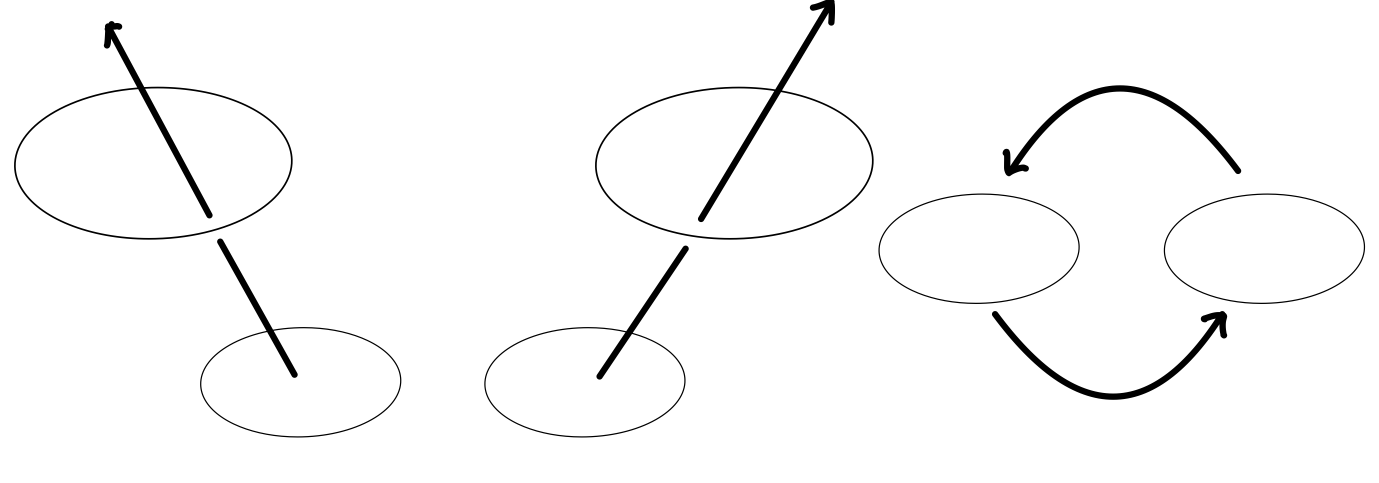
\includegraphics[width=0.8\textwidth]{images/welded_braids/0_welded_rings_crossings.png}
    \caption{Overcrossing (Left), Undercrossing (Centre), Virtual Crossing (Right)}
    \label{fig:welded_rings_overcrossing_undercrossing}
\end{figure}

\begin{Remark}
Let's consider our \( 4 \) dimensional braid, where each strand is a tube. 
Let's consider our fourth dimension as time, this implies that each frame of our movie visualisation is in \( [0, 1]^3 \) and our time component \( t \) is in \( [0, 1] \). 
Therefore for a given welded braid \( B \in wB_n \) we define.
\[ F_t(B) = \{ (x, y, z) \in [0, 1]^3 \mid (x, y, z, t) \in im(B) \} \]
Similarly to our classical braid visualisation, where we're intersecting the space where \( w = t \) with the image of \( B \). 

The intuition around this is that we're performing an intersection of a tube that is increasing in the \( w \) component with a space that's constant in the \( w \) component, and so each frame must be a ring embedded in \( [0, 1]^3 \). 
\end{Remark}

\subsection{The Welded Braid Group} \label{sec:w_group}

Let's consider the flying ring visualisation and consider the stacking of welded braids by performing one movie after another. 
I.e. we let \( A, B \in wB_n \) and define.
\[
AB := 
\begin{cases}
F_{2t}(A) &\text{for \( t \in [0, \frac{1}{2}] \)} \\
F_{2t - 1}(B) &\text{for \( t \in (\frac{1}{2}, 1]\)}
\end{cases}
\]
This forms a group, from which we can consider the Welded Braid Group described by \cite{Bar_Natan_2016}.

Let's consider the sequence of overcrossings, undercrossings, and virtual crossings in order of when they occurred in time. 
We will denote an overcrossing between strands \( i \) and \( i + 1 \) as \( \sigma_i \) and similarly an undercrossing between strands \( i \) and \( i + 1 \) as \( \sigma_i^{-1} \).
We will similarly denote a virtual crossing between strands \( i \) and \( i + 1 \) as \( s_i \). 
We can describe a welded braid \( B \in wB_n \) as a concatenation of the words \( \sigma_i, \sigma_i^{-1}, s_i \) for \( i \in [n - 1] \) where the order of words aligns with the sequence of crossings. 

This forms the group \( wB_n \) for any \( n \in \N \) and thus is a natural extension of \( uB_n \). 
Infact if we restrict welded braids such that virtual crossings do not occur, then the group formed by the stacking (performing a sequence of crossings and then another sequence of crossings) of welded braids is isomorphic to the our classical braid group with \( n \) strands \( uB_n \).
Therefore all our relations in \( uB_n \) are imposed on \( wB_n \).

We now impose relations pertaining to our virtual crossings.
\begin{align}
    s_i^2 &= 1 \label{eq:double_virtual_crossings} \\
    s_is_{i + 1}s_i &= s_{i + 1}s_i s_{i + 1} \\
    s_i s_j &= s_j s_i \quad \text{where } |i - j| > 1
\end{align}
And mixed relations.
\begin{align}
    s_i \sigma^{\pm 1}_{i + 1} s_i &= s_{i + 1} \sigma^{\pm 1}_{i} s_{i + 1} \\
    s_i \sigma_j &= \sigma_j s_i \quad \text{where } |i - j| > 1
\end{align}
There is one more relation which we haven't defined, it is called the \textit{Overcrossings commute} OC relation, and it breaks the symmetry between overcrossings and undercrossings. 
This is specifically interesting because it makes overcrossings and undercrossings fundamentally different.
\begin{equation}
    \sigma_i \sigma_{i + 1} s_i = s_{i + 1} \sigma_i \sigma_{i + 1} \label{eq:OC}
\end{equation}

\begin{Exercise}
    Describe what \cref{eq:double_virtual_crossings} and \cref{eq:OC} represent in their flying rings visualisation. 
\end{Exercise}
\begin{Exercise}
    We call a classical braid \textsc{pure} if the skeleton of the braid (braid without crossing information and thus is a permutation) is the identity permutation. 
    For example, the skeleton of \( \sigma_1 \sigma_2 \in uB_3 \) is \( (1 2)(2 3) = (1 3 2) \in \mathbb{S}_3 \) which isn't the identity and so \( \sigma_1 \sigma_2 \) isn't a pure braid. 
    
    Describe pure welded braids in terms of the flying ring visualisation of welded braids.
\end{Exercise}
\begin{Exercise} \label{ex:UC}
    Using the flying rings visualisation, explain why the \textsc{Undercrossings Commute} UC relation \( s_i \sigma_{i + 1} , \sigma_i = \sigma_{i + 1} \sigma_i s_{i + 1} \) is false. 
\end{Exercise}

\subsection{Welded Braid Diagrams}

Our classical braid diagram took advantage of a projection with extra information, for welded braids this doesn't extend nicely and thus we will define our welded braid diagrams artificially by denoting overcrossings and undercrossings the same as classical braids, however denoting virtual crossings as

% Virtual crossing diagram picture.
\begin{figure}[H]
    \centering
    
\includegraphics[width=0.15\textwidth]{images/welded_braids/1_welded_virtual_crossing.png}
    \caption{Virtual Crossing}
    \label{fig:virtual_crossing}
\end{figure}

We will denote the number of crossings of a braid \( B \) as \( k_B \). 
We will consider the base of the diagram as being height \( 0 \) and the top of the diagram as being height \( 1 \). 
Consider \( B \in wB_n \) and \( k_B \) values of height linearly spaced along \( [0, 1] \), i.e. \( h_B = \left\{ \frac{i}{k_B + 1} \in [0, 1] \mid i \in [k_b] \right\} \).
We will consider a crossing to occur instantaneously at these height values in the order in which they occur as a sequence of crossings. 
I.e. if \( \sigma_i \) is the \( k \)th crossing to occur for a braid \( B \), then we place the diagram of \( \sigma_i \) between the \( i \) and \( i + 1 \)th braids. \label{par:wb_diagram}

Therefore for a given braid diagram we can determine the information about the sequence of crossings of the braid by considering the order from bottom to top of which crossings occur. 
We then consider the braid diagram under isotopy, subject to the welded braid relations described in \cref{sec:w_group}. 

We therefore have an equivalence between the flying rings visualisation, the group, and the braid diagram of welded braids. 
\begin{Example}
    Let \( A = \sigma_1 s_2 \sigma_2 \in wB_3 \) and \( B = s_1 s_2 \sigma^2_2 \in wB_3 \). 
    Their braid diagram are described by
    \begin{figure}[H]
        \centering
        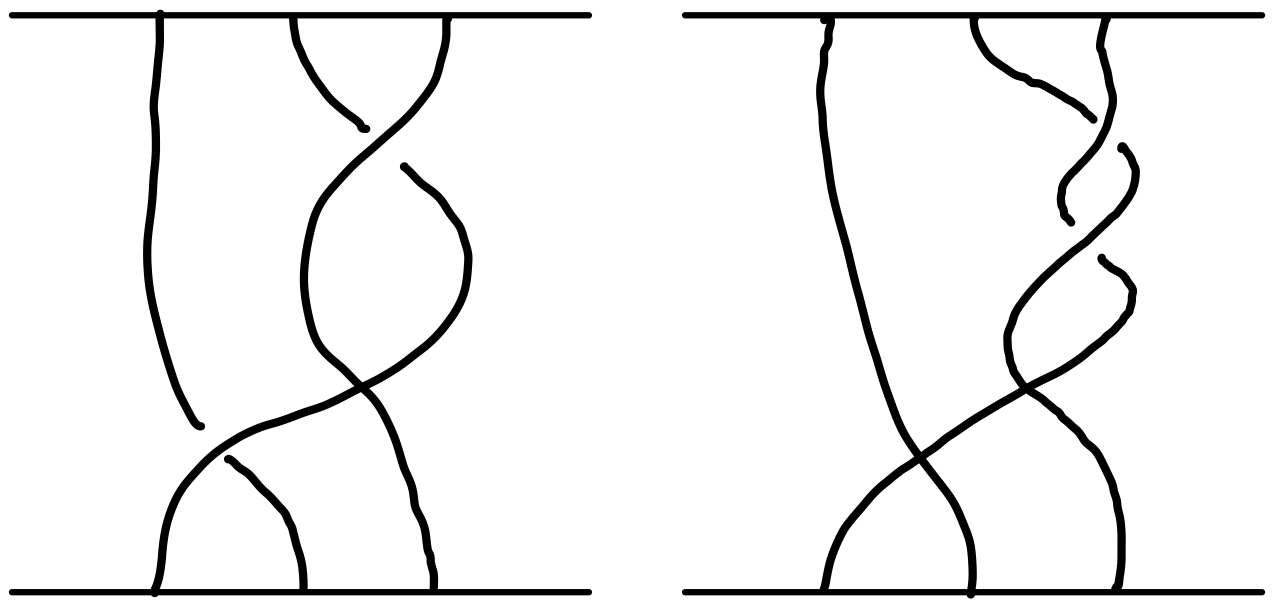
\includegraphics[width=0.8\textwidth]{images/welded_braids/2_welded_diagrams_example.png}
        \caption{\( A \) (left) and \( B \) (right)}
    \end{figure}
\end{Example}
\begin{Exercise}
    Determine the skeleton and braid diagram for the braids described by \( \sigma_1 s_1 s_2 \in wB_3 \) and \( \sigma_2 s_2 \sigma^{-1}_1 \sigma_1 s_1 \in wB_3 \).
\end{Exercise}
\begin{Exercise}
    Show that OC is equivalent to \( \sigma_i^{-1} s_{i + 1} \sigma_i = \sigma_i s_i \sigma_{i + 1}^{-1} \) algebraically, then by considering the braid diagram and flying rings visualisation. 
\end{Exercise}
